\documentclass[11pt]{article}

\usepackage[T1]{fontenc} % ensure scalable (Type1) fonts for pdfTeX/microtype expansion
\usepackage{lmodern}     % Latin Modern: Type1 versions of Computer Modern

\usepackage[margin=1in]{geometry}
\usepackage{amsmath,amssymb,amsfonts,amsthm}
\usepackage{mathtools}
\usepackage{bm}
\usepackage{hyperref}
\usepackage{graphicx}
\usepackage{enumitem}
\usepackage{booktabs}
\usepackage{microtype}
\usepackage{tcolorbox}
\usepackage{tabularx}
\usepackage{caption}
\usepackage[table]{xcolor}
\definecolor{groupgray}{RGB}{235,235,235} % change to any solid color you like


% Define a custom environment that behaves like a beamer block
\newtcolorbox{block}[1]{
  colback=blue!5!white,
  colframe=blue!75!black,
  title=#1
}
\usepackage{authblk}
\title{Mitigating Adverse Selection in Concentrated Liquidity AMMs with Dynamic Fees: An Agent-Based Model Approach\\[0.3em]
\large \textit{Extended Abstract}}
\author[1]{Daniele Maria Di Nosse}
\author[1]{Fabrizio Lillo\footnote{FL acknowledges support from
the grant PRIN2022 DD N. 104 of February 2, 2022 ”Liquidity and systemic risks in centralized and decentralized markets”,
codice proposta 20227TCX5W - CUP J53D23004130006 funded by the European Union NextGenerationEU through the Piano
Nazionale di Ripresa e Resilienza (PNRR).}}

\affil[1]{Scuola Normale Superiore, Pisa, Italy}
\date{\today}

\begin{document}

\maketitle

\section{Introduction}
Automated market makers (AMMs) have become a foundational market design for decentralized finance (DeFi), enabling 
permissionless exchange without centralized limit order books in decentralized exchanges (DEXs). Uniswap v3 is a pivotal 
step in this evolution: by introducing concentrated liquidity, it allows liquidity providers (LPs) to allocate capital 
within chosen price intervals rather than uniformly over the entire price axis \cite{adams2021}.
This design markedly increases capital efficiency and can improve execution quality for traders near the prevailing price. 
At the same time, it fundamentally changes LP risk: concentrated positions behave like short-volatility portfolios whose 
inventory becomes progressively one-sided when price trends, and whose profitability depends on earning sufficient fees
to compensate for adverse selection and re-hedging costs. In this context, recent theoretical work has clarified that 
what matters economically is not raw mark-to-market performance, but hedged profitability, often expressed as 
Fees - Loss-Versus-Rebalancing (LVR) \cite{milionis2023}. LVR formalizes the systematic loss suffered by passive liquidity provision 
when arbitrageurs trade against stale AMM prices after an external reference price moves. This paper contributes a 
granular agent-based modeling framework based on the Uniswap v3 dynamics and designed to study exactly this 
interplay—between concentrated-liquidity mechanics, blockchain execution frictions, heterogeneous strategic behavior, and fee 
design—under controlled and interpretable conditions. The results extend to all the concentrated-liquidity AMM designs that share
Uniswap v3’s core mechanics. 


\section{Motivation and research question}

The empirical and theoretical literature increasingly suggests that, for volatile pairs, passive LPing in Uniswap v3 often yields negative outcomes relative 
to simple holding, and even more starkly negative outcomes on a hedged basis, see, for example, \cite{fritsch2024}, \cite{heimbach2022}, \cite{cohen2023}, \cite{cartea2023}. 
The core mechanism is adverse selection: when prices move quickly, arbitrageurs “pick off” AMM quotes, transferring value from LPs to arbitrageurs. Yet most analytical models
necessarily simplify the execution layer, as they often assume continuous time, frictionless adjustment, or abstract the discrete block structure that 
characterizes blockchain settlement. Meanwhile, protocol practice is evolving: several major AMM designs now implement dynamic fees that respond endogenously 
to volatility, imbalance, or activity regimes. However, how dynamic fees interact with realistic microstructure frictions (block latency, stochastic ordering, mempools) 
and strategic agents such as rational routers, Maximal Extractable Value (MEV) searchers \cite{flashboys} and active LPs remains under-explored.

The central question of this work is therefore:

Can dynamic taker-fee schedules improve the economic sustainability of concentrated-liquidity provision—measured by positive hedged LP PnL, without destroying the DEX’s 
competitiveness, and how do these conclusions change once active LP behavior and more sophisticated strategies such as Just-In-Time (JIT) liquidity \cite{wan2022just} are introduced? 

\section{Main contributions}

This paper’s primary contribution is the study of dynamical fee schedule for concentrated-liquidity AMMs through an Agent-Based Model (ABM).
Relative to much of the existing DeFi/AMM ABM literature---where models are often built around constant-product pools and simplified agent populations (see for instance \cite{angeris2021analysisuniswapmarkets})---
we (i) implement Uniswap v3 mechanics explicitly and (ii) couple them to a richer, microstructure-aware agent ecology. 
This controlled setting then allows us to isolate, in counterfactual experiments, the effect of several dynamic taker-fee rules on both LP economics and DEX competitiveness. 
The full simulator and scripts to reproduce the figures are available in our public repository \cite{abm_uni_v3_repo}.
The main characteristics of the model can be summarized as follows:

\begin{itemize}
    \item Uniswap v3-specific AMM mechanism: The market dynamics is implemented on a discrete tick grid with concentrated 
    liquidity, and pathwise (tick-by-tick) swap execution with fee accrual. To the best of our knowledge, ABMs that explicitly 
    model v3’s concentrated-liquidity accounting remain rare.
    \item Rich agent ecology and blockchain microstructure: Time advances in blocks with within-block order arrival, 
    mempool accumulation, and stochastic ordering at block close. The ecosystem includes arbitrageurs, noise traders, a 
    best-execution smart router, passive and active LP cohorts with budgets and 
    review clocks to prevent synchronization, and an MEV-style JIT liquidity provider.
    \item Controlled evaluation of dynamic fee rates: Within the same microstructure and agent ecology, we compare multiple 
    implementable fee controllers (volatility-based and toxicity/staleness-based), subject to bounds, hysteresis, and 
    step-size limits, and quantify their impact on Fees, LVR, hedged LP PnL, routed DEX share, and fee incidence under JIT.
    \item Discrete-time LVR benchmark for v3 LPs: For each LP, the model constructs a self-financing rebalancing benchmark 
    that matches inventory but trades at the reference price, yielding the identity Hedged PnL = Fees - LVR in a block-based simulation \cite{milionis2023}. 
\end{itemize}

Together, these components allow experiments that connect protocol levers (fees, liquidity concentration, execution frictions) to economic outcomes 
(hedged LP profits, arbitrage extraction, routing share, MEV redistribution).

\section{Model}

The AMM trades two tokens: token 0 and token 1 against each other. Prices evolve on a discrete tick grid, with tick $i$ 
mapped to square-root price via $s_t=1.0001^{\frac{i}{2}}$. Liquidity positions are intervals ($[i_a,i_b]$), 
contributing to total active liquidity when the current tick lies in that interval. The pair composed by active liquidity 
and square-root prices determine the current state of the pool. Swaps are executed within ticks using the v3 algebra, and large 
trades are executed pathwise across ticks: liquidity updates at tick boundaries via the net-liquidity map that tracks how much 
liquidity must be added and removed from the current active liquidity when crossing to a new tick, producing piecewise price impact. 
Fees are charged on the input side and distributed pro-rata to LPs active over the traversed region. 

The simulator operates in discrete blocks ($t=1,\dots,T$), each containing ($B$) micro-steps. Agents observe the last validated on-chain snapshot at 
the beginning of a block; during micro-steps, the reference price evolves but the on-chain state is effectively stale from the agents’ perspective. All 
agent actions generate “intents” appended to a mempool. At the block boundary, the simulator executes a mempool replay: it shuffles transactions to 
represent stochastic ordering, executes an arbitrage intent with priority, and then executes remaining intents sequentially. This creates a latency 
wedge between information and execution and reproduces a key microstructure feature: within-block reference price moves can create transient mispricings that 
become arbitrage opportunities at block close. 

The CEX mid-price ($m_t$) follows a Heston stochastic volatility specification, generating time-varying variance ($v_t$) and correlated shocks. This 
allows the ABM to test fee controllers under volatility clustering rather than constant-volatility baselines. Additionally, net signed CEX volume 
produces permanent impact through a concave power law in executed volume, introducing feedback from arbitrage execution into the reference dynamics. 

\subsection{LVR and hedged profitability}

A central methodological piece is the discrete-time rebalancing benchmark used to compute LVR coherently in a block-based simulation. Each LP has 
mark-to-market wealth ($V^{LP}_t = x_t m_t + y_t$), where ($x_t$) is token-0 exposure (aggregated across opened positions) and ($y_t$) is token-1 cash. 
A benchmark portfolio is constructed to satisfy:
\begin{itemize}
    \item Inventory matching: it always holds ($x^{reb}_t = x_t$).
    \item Self-financing: adjustments in token-0 exposure are financed by token-1 at the CEX mid price.
    \item Execution at fresh prices: the benchmark’s rebalancing trades occur at ($m_t$), not at the AMM’s stale execution price.
\end{itemize}

This yields the decomposition identity enforced in the model:
\begin{equation}
    V^{LP}_t = V^{reb}_t + F_t - LVR_t,
\end{equation}
and hence
\begin{equation}
\Pi^{hedged}_t = V^{LP}_t - V^{reb}_t = F_t - LVR_t.    
\end{equation}

The hedged PnL isolates the economic “alpha” of liquidity provision: it cannot be inflated merely by taking more directional exposure, 
because any exposure path affects both the LP and benchmark in lockstep. 

\subsection{Agent ecology}

\paragraph{Arbitrageurs.}

Arbitrageurs act on each block to exploit DEX–CEX discrepancies subject to wedges from the taker fee and a flash-loan funding cost. They choose 
trade size to push the post-trade marginal DEX price to the boundary of the no-arbitrage band. This creates realistic size dependence: arbitrage 
does not merely “snap” the pool price to the reference; it interacts with finite depth and the tick liquidity profile. Arbitrage is executed with 
priority in the mempool replay, approximating MEV ordering advantages. 

\paragraph{Liquidity providers: passive and active cohorts.}

LPs are cash-budgeted in token 1 and mint/burn Uniswap v3 positions based on strategy-specific rules, subject to review 
clocks and cooldowns periods that prevent synchronization across all the LPs. Specifically, each LP has two internal 
clocks that determine when it is possible to act and how long it must wait before it can become operate again. Passive 
LPs mint and burn according to a fixed probability per block. They choose wide ranges an center them around the current 
price. Active LPs perform actions according to fixed probability per block as well, but they concentrate 
liquidity much more around the current price, using volatility-related signals to adapt range width, 
and implement recentering when price moves out of range as well as simple take-profit/stop-loss triggers. Because narrower 
ranges increase marginal liquidity around the price, active LPs are expected to collect a higher fee density but also to 
suffer a higher LVR per unit time—precisely the trade-off studied in the simulations. 

\paragraph{Liquidity takers: noise trader and smart router}

The model includes two complementary sources of order flow:

\begin{itemize}
    \item A noise trader who submits random-direction swaps with lognormal size and a slippage constraint, representing uninformed or urgency-driven 
    flow that pays fees and generates volume but can create mispricings harvested by arbitrage. 
    \item A smart router that compares quotes from the AMM and CEX and routes each trade to the venue offering the best price (subject to slippage tolerance). 
    This agent is crucial for endogenizing DEX market share: when fees rise or liquidity thins, routed volume migrates to the CEX, decreasing fee 
    revenue to LPs and altering equilibrium profitability. 
\end{itemize}

\paragraph{JIT liquidity provider (Jiter).}

In the most complex model, a JIT searcher targets the largest pending swap (by notional) and “wraps” it with a one-tick position: 
mint → swap executes against it → burn immediately. The Jiter’s sizing trades off expected fee capture against flash-financing cost, 
and it caps its share of in-tick liquidity. This agent captures a stylized but economically central MEV dynamic: fee revenue that would 
have accrued to longer-horizon LPs can be gained by ultra-short-lived liquidity posted exactly at execution. 

\section{Dynamic fee schedules}

The paper evaluates fee dynamics through a set of simple, implementable controllers updated on a block clock. The fee is 
bounded between a floor and a cap; changes are gated by a minimum-change threshold and a cooldown between fee updates, 
and are further limited by a maximum per-update step size, preventing rapid oscillations. Within that infrastructure,  
the study focuses on two main signal families:

\begin{itemize}
    \item Volatility-based fees: the fee reacts to an Exponential Weighted Moving Average (EWMA) of realized volatility 
    (defined on either CEX or validated DEX returns), increasing with volatility. 
    \item Toxicity-based fees: the controller measures “excess basis” by comparing the absolute log DEX--CEX gap to the 
    current fee band. Only deviations beyond the fee wedge contribute to the signal, which is then smoothed and mapped 
    into fee increases. This is designed to respond directly to the microstructural condition that generates LVR: 
    the extent to which the AMM is stale relative to the reference beyond what fees already compensate. 
\end{itemize}


\section{Results}
We study three variants of increasing strategic complexity:
\emph{Model~0} (passive LPs + arbitrageur + noise trader + router),
\emph{Model~1} (add active LPs),
\emph{Model~2} (add Jiter).
Simulations run over long horizons and results are aggregated across multiple runs. We report hedged LP PnL, DEX market 
share (fraction of trades routed to the DEX), fee distributions, and arbitrage diagnostics to ensure that observed 
differences are not artifacts of arbitrage breakdown.

\subsection*{Fixed fees}
With constant taker fees, hedged LP PnL is persistently negative across all three models. Even when routed flow is 
significant---in Model~2 the median DEX market share is around $43\%$---fee revenue fails to compensate LVR created by 
block-latency-induced mispricings. Concentration amplifies losses: in Model~1, active (narrow-range) LPs perform worse 
than passive LPs on a hedged basis, consistent with the concentration--LVR trade-off. In short, a fixed fee behaves like 
a fixed spread applied to a market maker whose quotes cannot be refreshed continuously; it underprices adverse selection
 in stressed blocks and overprices benign flow in calm blocks.

\subsection*{Dynamic fees without JIT}
Dynamic fees change the balance by widening the no-arbitrage band when staleness is high, reducing profitable 
arbitrage and increasing LP compensation in exactly those blocks.
In Model~0, the toxicity controller makes hedged PnL for passive LPs persistently positive over the full horizon 
while keeping fee levels and activity plausible: the upper quartile of fees is around $0.1\%$ (with rare excursions 
above $1\%$) and routed DEX share stabilizes around $25\%$ rather than collapsing to zero. Arbitrage diagnostics align 
with this interpretation: executed arbitrage trades drop substantially relative to the fixed-fee baseline (roughly from 
$\sim 9{,}020$ to $\sim 5{,}843$ arbitrage swaps per run in our baseline parametrization), consistent with a widened 
fee-implied band that renders fewer discrepancies profitable to exploit.

Volatility-based schedules also improve passive outcomes, but their gains are weaker and less robust across configurations 
with respect to the toxicity fee specification. The reason is microstructural: volatility is only an indirect proxy for 
 adverse selection in a block-time execution environment. Volatility can be high while arbitrage keeps the pool close to 
 the reference (small gaps), and volatility can be moderate  while ordering and latency still produce transient staleness 
 in specific blocks. In Model~1, this becomes decisive: the toxicity-driven schedule is the only tested controller under 
 which both passive and active LP cohorts achieve positive hedged profits. Volatility-driven controllers can move passive 
 LPs toward break-even but leave active LPs negative, indicating that in concentrated-liquidity regimes fees must respond 
 to realized toxicity rather than to broad time-varying volatility.

Figure~\ref{fig:main_results_model0} visualizes these effects for the baseline case without JIT liquidity (Model~0).

\begin{figure}[t]
    \centering
    \begin{minipage}[t]{0.49\linewidth}
        \centering
        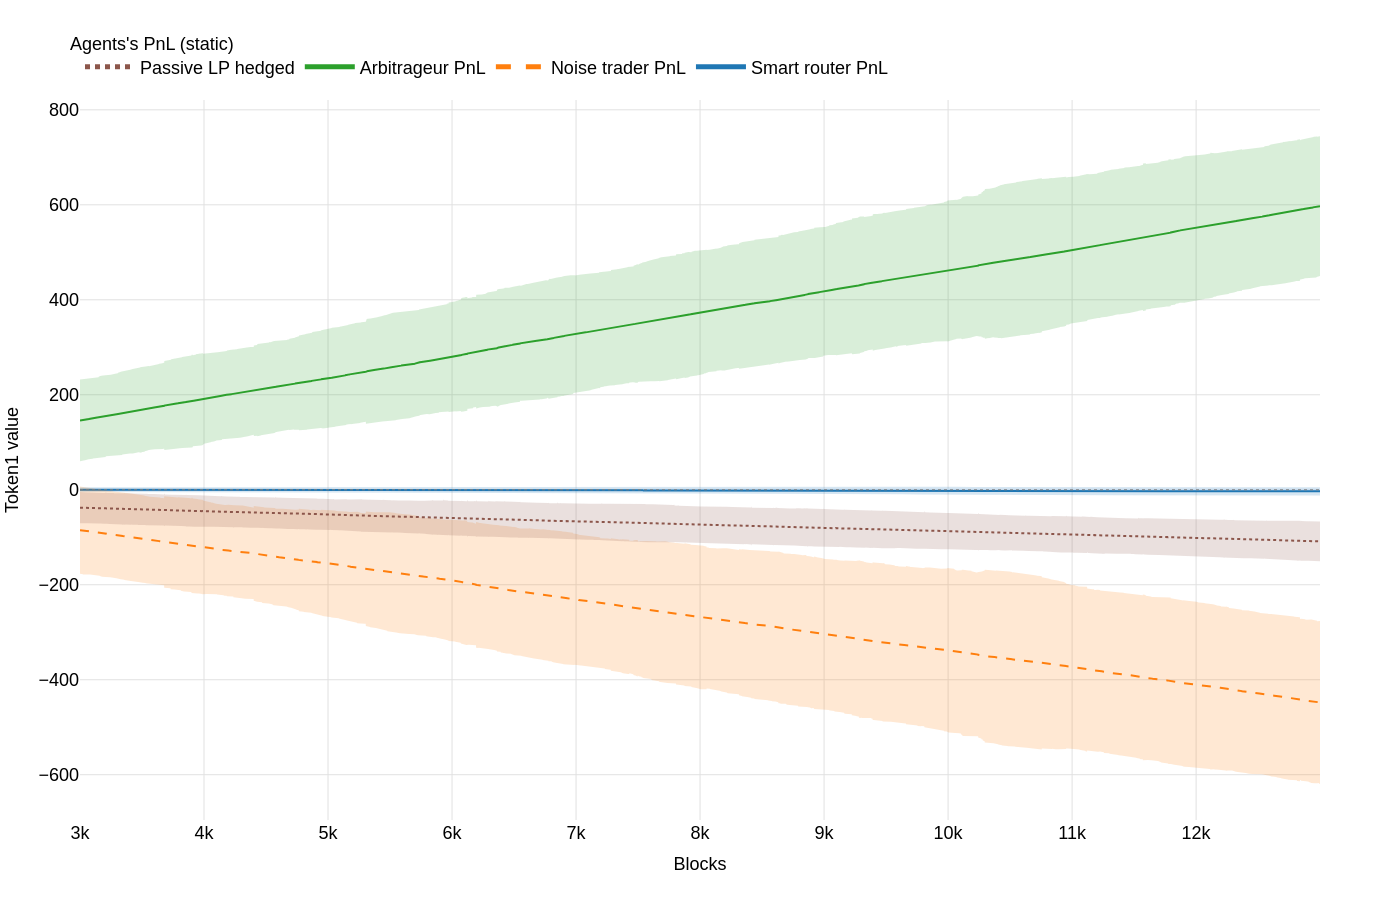
\includegraphics[width=\linewidth]{images/pnl_static_test_runs50_LPpassiveshare1_pjit0_293410.png}
        \par\small\textbf{(a)} Fixed (static) taker fee.
    \end{minipage}\hfill
    \begin{minipage}[t]{0.49\linewidth}
        \centering
        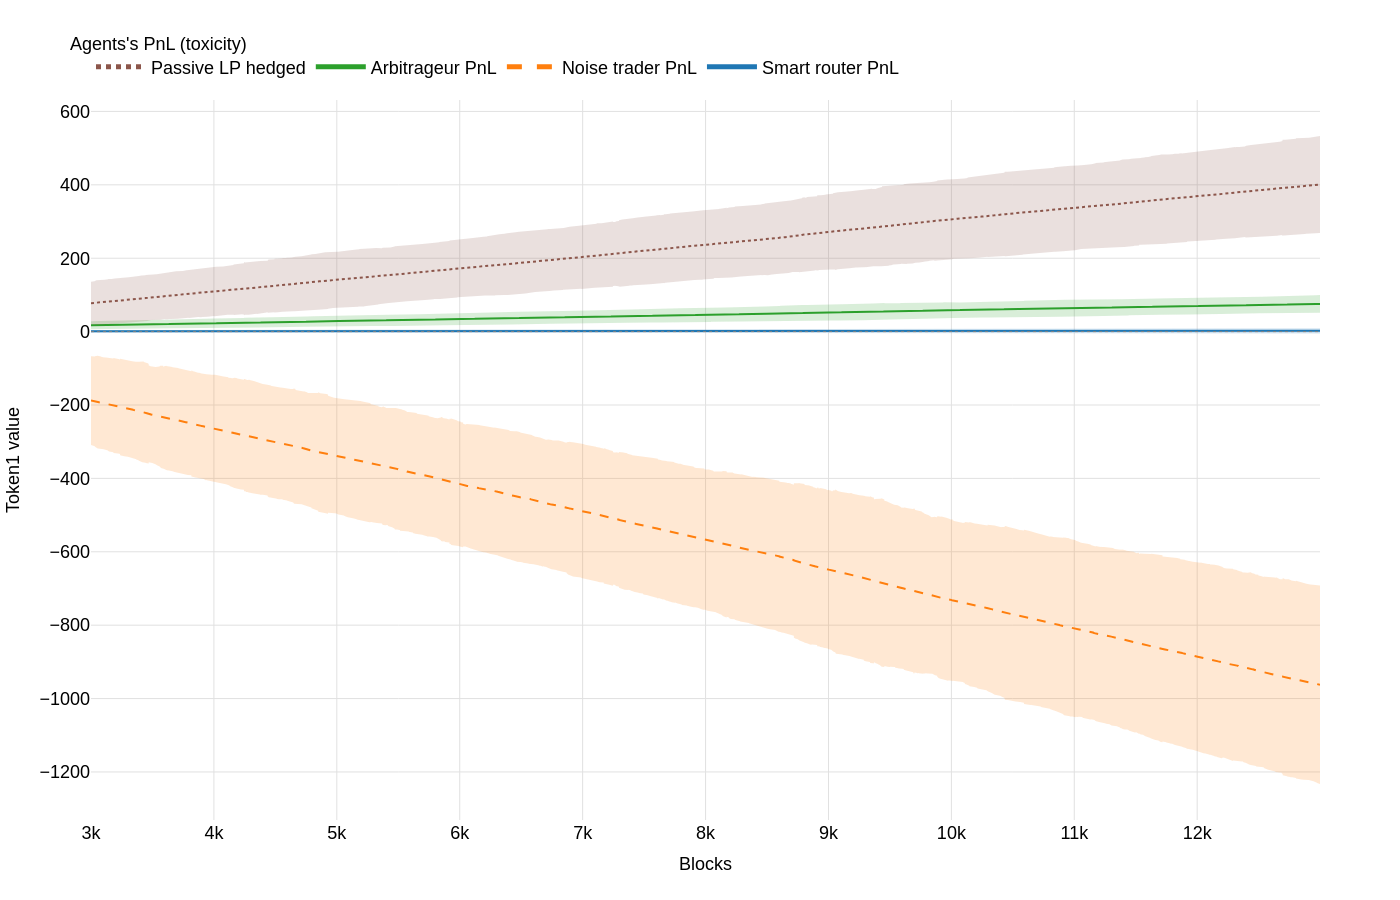
\includegraphics[width=\linewidth]{images/pnl_toxicity_test_runs50_LPpassiveshare1_pjit0_293410.png}
        \par\small\textbf{(b)} Toxicity-driven dynamic fee.
    \end{minipage}

    \medskip
    \begin{minipage}[t]{0.85\linewidth}
        \centering
        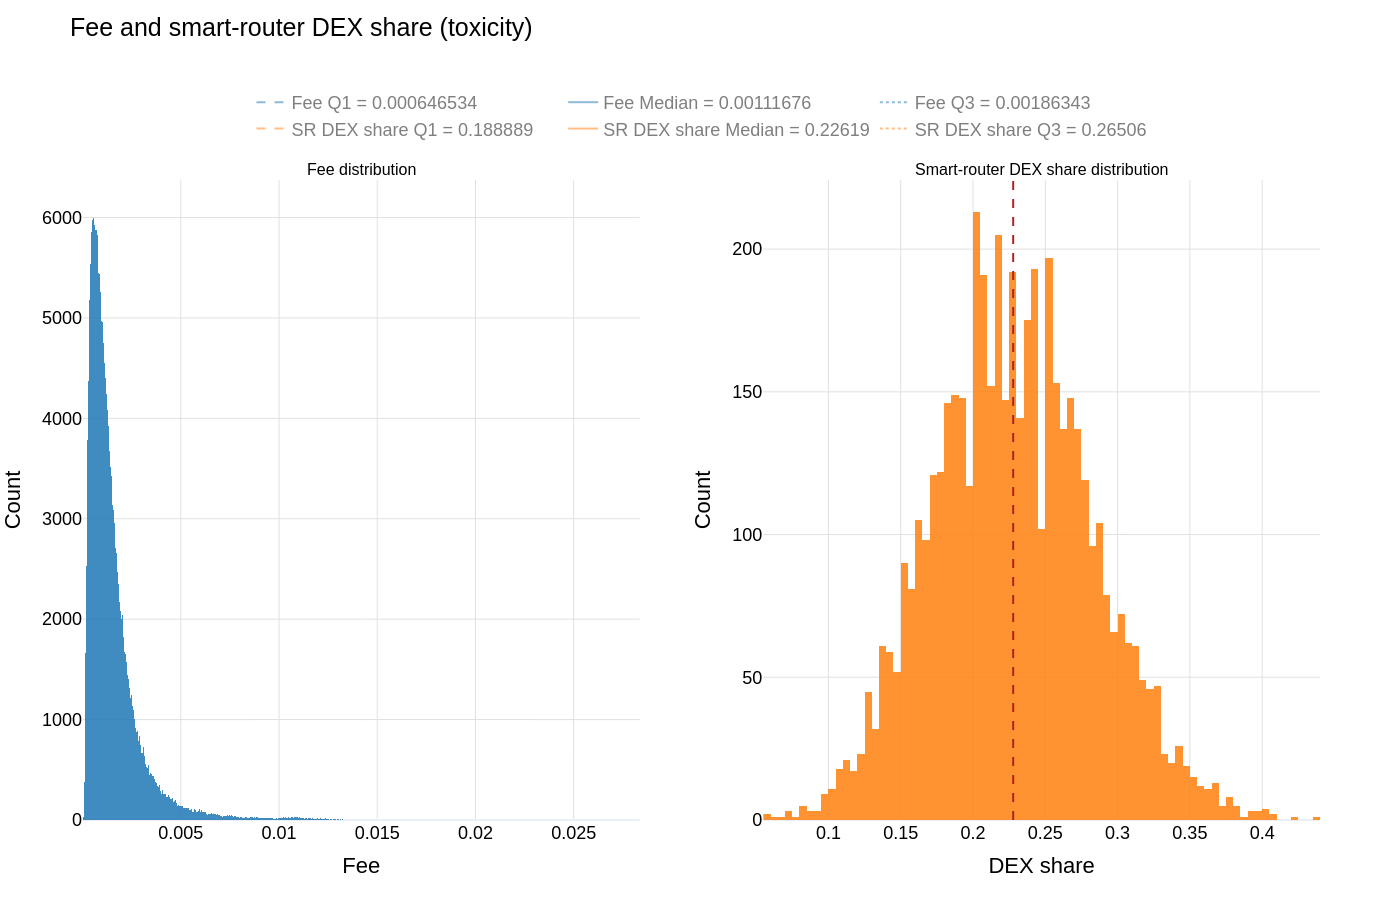
\includegraphics[width=\linewidth]{images/fee_toxicity_test_runs50_LPpassiveshare1_pjit0_293410.png}
        \par\small\textbf{(c)} Fee and routed DEX share distribution (toxicity controller).
    \end{minipage}
    \caption{Illustrative summary of the main result without JIT (Model~0). Under fixed fees (panel a) passive LPs exhibit persistently negative hedged PnL (Fees $-$ LVR). A toxicity-driven controller (panel b) adapts fees to block-time staleness and can restore positive hedged LP profitability while maintaining non-zero routed DEX market share (panel c). Curves are averaged across 50 runs; shaded bands correspond to $\pm 2$ standard deviations.}
    \label{fig:main_results_model0}
\end{figure}

\subsection*{LVR behavior and fee coverage}
To connect hedged profitability to its microstructural driver, we study how Loss-Versus-Rebalancing (LVR) accumulates at block frequency as the block time $B$ changes. LVR theory implies that, holding other frictions fixed, adverse selection costs scale with the variance of the reference price over the stale-quote window, i.e., approximately as $\sigma^2 \Delta t$ \cite{milionis2023}. In our simulator, increasing $B$ lengthens the within-block period during which the DEX can be stale relative to the CEX, and therefore increases typical per-block LVR increments.

A compact diagnostic is the fee-coverage ratio
\[
    r_t = \frac{\Delta \mathrm{LVR}_t}{\Delta F_t},
\]
where $\Delta \mathrm{LVR}_t$ and $\Delta F_t$ denote per-block increments of LVR and fees. Values $r_t>1$ indicate that, at the block margin, fee revenue is insufficient to compensate adverse selection, implying negative hedged LP PnL on average.
Figure~\ref{fig:lvr_fee_coverage} reports the median $r_t$ over a block-time sweep. Under static fees, $r_t$ exceeds one and increases with $B$, consistent with fixed fees underpricing block-time adverse selection. Under toxicity-driven fees, the ratio decreases substantially and becomes more stable across $B$, with medians closer to (and often below) one, consistent with the controller aligning fee income with realized staleness.

\begin{figure}[t]
  \centering
  \begin{minipage}[t]{\linewidth}
    \centering
    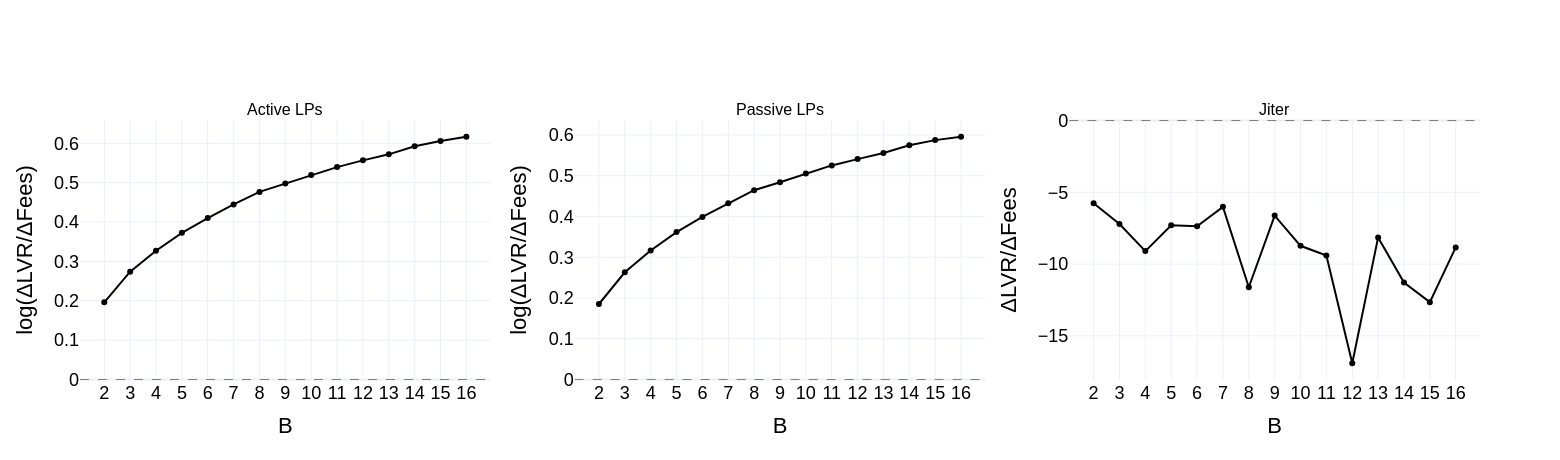
\includegraphics[width=0.95\linewidth]{images/dLVR_over_dFees_medians_vs_block_time_static_flow_test_runs50_pid42657.png}
    \par\small\textbf{(a)} Static fees.
  \end{minipage}

  \vspace{0.6em}

  \begin{minipage}[t]{\linewidth}
    \centering
    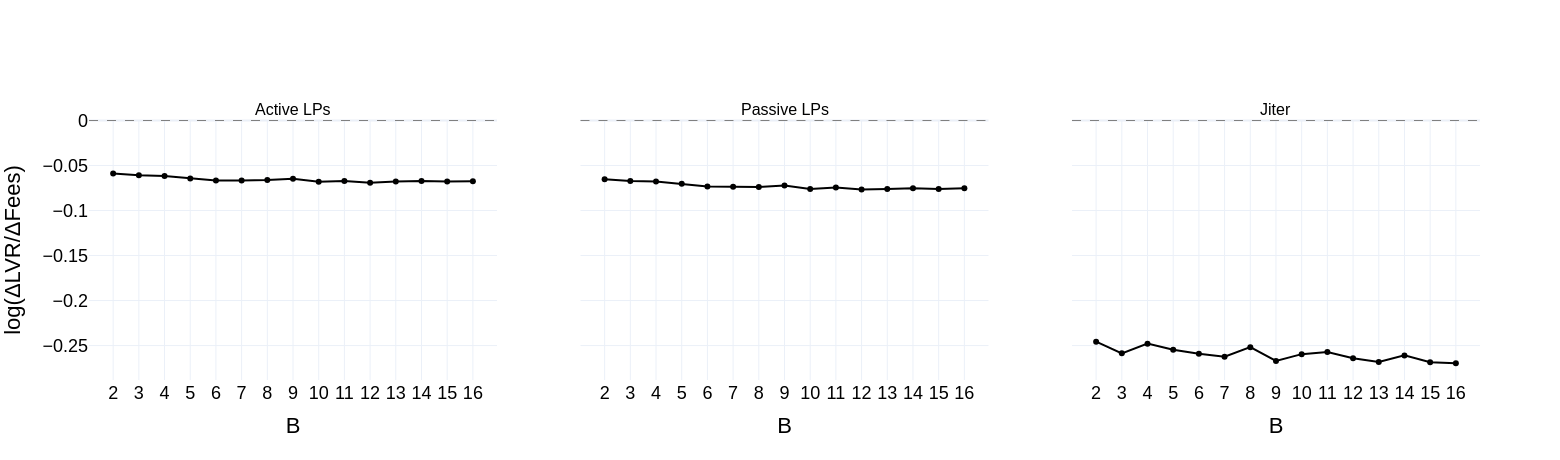
\includegraphics[width=0.95\linewidth]{images/dLVR_over_dFees_medians_vs_block_time_toxicity_flow_test_runs50_pid14207.png}
    \par\small\textbf{(b)} Toxicity-driven fees.
  \end{minipage}

  \caption{Median fee-coverage ratio $r_t=\Delta \mathrm{LVR}_t/\Delta F_t$ as a function of block time $B$ in a block-time sweep experiment. Ratios above one indicate that adverse selection (LVR) dominates fee income at the margin. Medians are computed across runs (with dispersion bands shown in the underlying plots).}
  \label{fig:lvr_fee_coverage}
\end{figure}

\subsection*{Dynamic fees with JIT}
Model~2 exposes a second tension. Once JIT liquidity is allowed, adaptive fees make the JIT strategy profitable: the
searcher enters precisely when fees spike, captures a dominant fraction of the fee mass around the largest swap, and 
exits immediately, keeping inventory risk minimal. In our experiments, this diversion of fee revenue prevents ordinary
LP cohorts from reaching positive hedged PnL under any tested dynamic schedule. Importantly, arbitrage-related counts
remain broadly stable across specifications, indicating that the deterioration for non-JIT LPs is best understood as
fee incidence (who earns the fees) rather than a resurgence of arbitrage intensity. Economically, the mechanism
 is coherent: the controller increases the fee ``prize'' in precisely those blocks that trigger JIT entry, and a 
 latency/priority-advantaged agent can appropriate that prize while leaving longer-horizon LPs exposed to residual
 stale-quote risk.

Figure~\ref{fig:main_results_model2_jit} illustrates this fee-incidence shift once JIT liquidity is introduced (Model~2).

\begin{figure}[t]
    \centering
    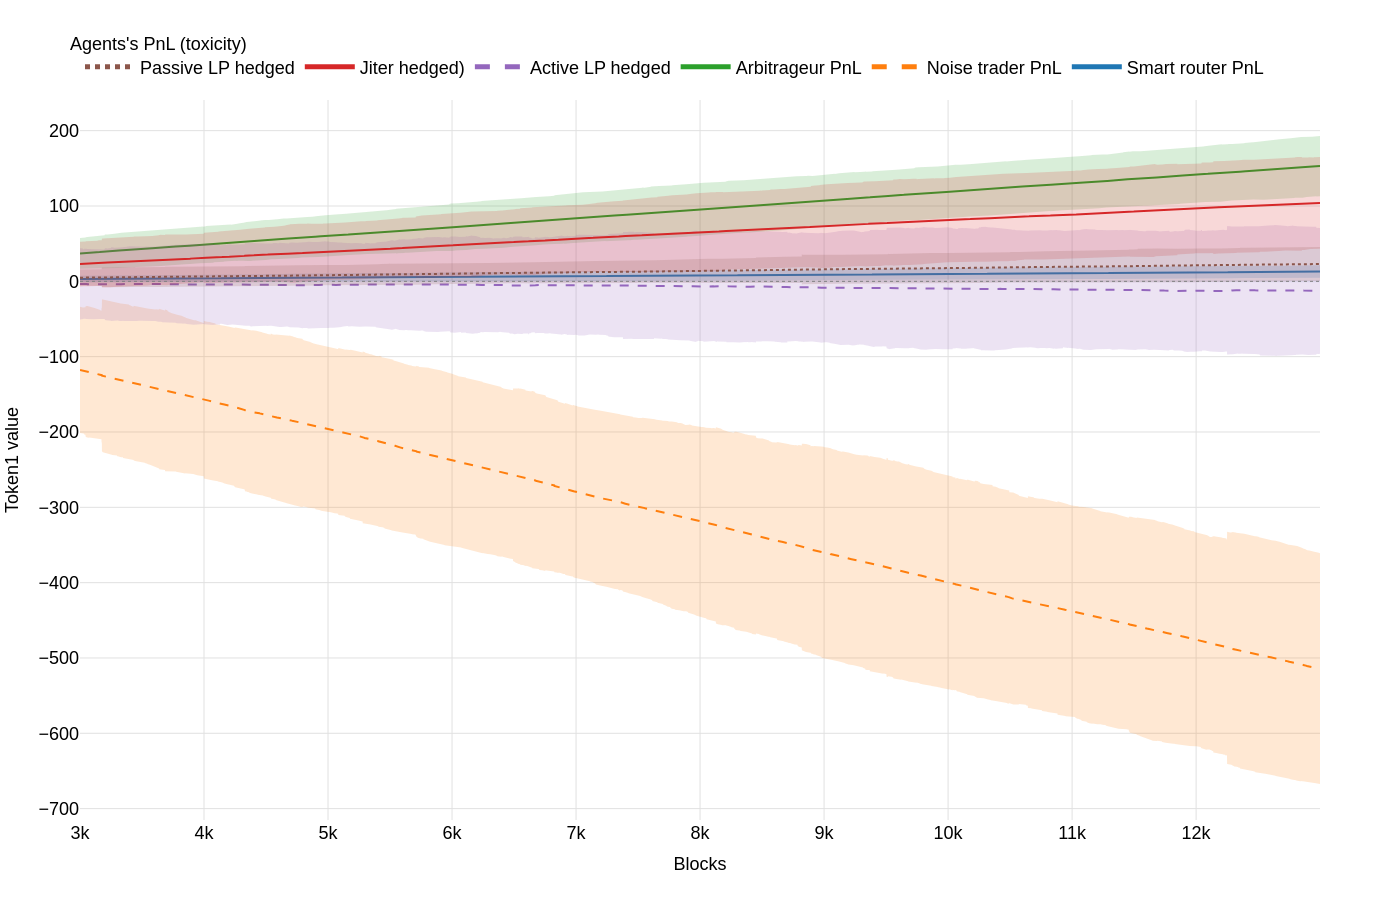
\includegraphics[width=0.85\linewidth]{images/pnl_toxicity_test_runs50_LPpassiveshare0.5_pjit1_102248.png}
    \caption{Dynamic fees with JIT (Model~2). Under toxicity-driven fee adaptivity, the JIT liquidity provider (Jiter) can extract positive hedged PnL by supplying one-block liquidity precisely when fees spike, while longer-horizon LP cohorts remain negative on a hedged basis. Curves are averaged across 50 runs; shaded bands correspond to $\pm 2$ standard deviations.}
    \label{fig:main_results_model2_jit}
\end{figure}

\section{Discussion}
Three conclusions follow for concentrated-liquidity AMMs operating under realistic blockchain microstructure. First, LVR
is deeply microstructural: block latency and ordering create stale-quote windows that act as a systematic adverse selection
tax on LPs. Second, dynamic fees can internalize this tax, but only if the control signal is aligned with the structural 
driver (staleness/toxicity) rather than with broad volatility states. Third, MEV/JIT can dominate fee incidence: fee 
adaptivity that protects LPs in a no-JIT world can backfire once liquidity is allowed to appear for a single block to 
capture elevated fees.

A natural extension is therefore joint mechanism design: fee adaptivity together with MEV-resilience and/or fee 
attribution rules that reward liquidity persistence (e.g., time-weighted fee allocation, cooldowns, or penalties for 
flash-funded mint/burn cycles). More broadly, the ABM provides a laboratory for comparing such proposals under controlled
and interpretable microstructure frictions, and for connecting protocol levers (fees, execution rules) to economic 
outcomes (hedged LP profits, arbitrage extraction, routed market share, and MEV redistribution).

\bibliographystyle{abbrv}
\bibliography{extended_abstract}

\end{document}
